\hypertarget{rn__init_8c}{
\section{rn\_\-init.c File Reference}
\label{rn__init_8c}\index{rn_init.c@{rn\_\-init.c}}
}


\subsection{Detailed Description}
\begin{Desc}
\item[For internal use only.]
This file contains the implementation of the \hyperlink{group__dbprim__rbtree_ga14}{rn\_\-init()} function, used to dynamically initialize a red-black tree node.\end{Desc}


Definition in file \hyperlink{rn__init_8c-source}{rn\_\-init.c}.

{\tt \#include \char`\"{}dbprim.h\char`\"{}}\par
{\tt \#include \char`\"{}dbprim\_\-int.h\char`\"{}}\par


Include dependency graph for rn\_\-init.c:\begin{figure}[H]
\begin{center}
\leavevmode
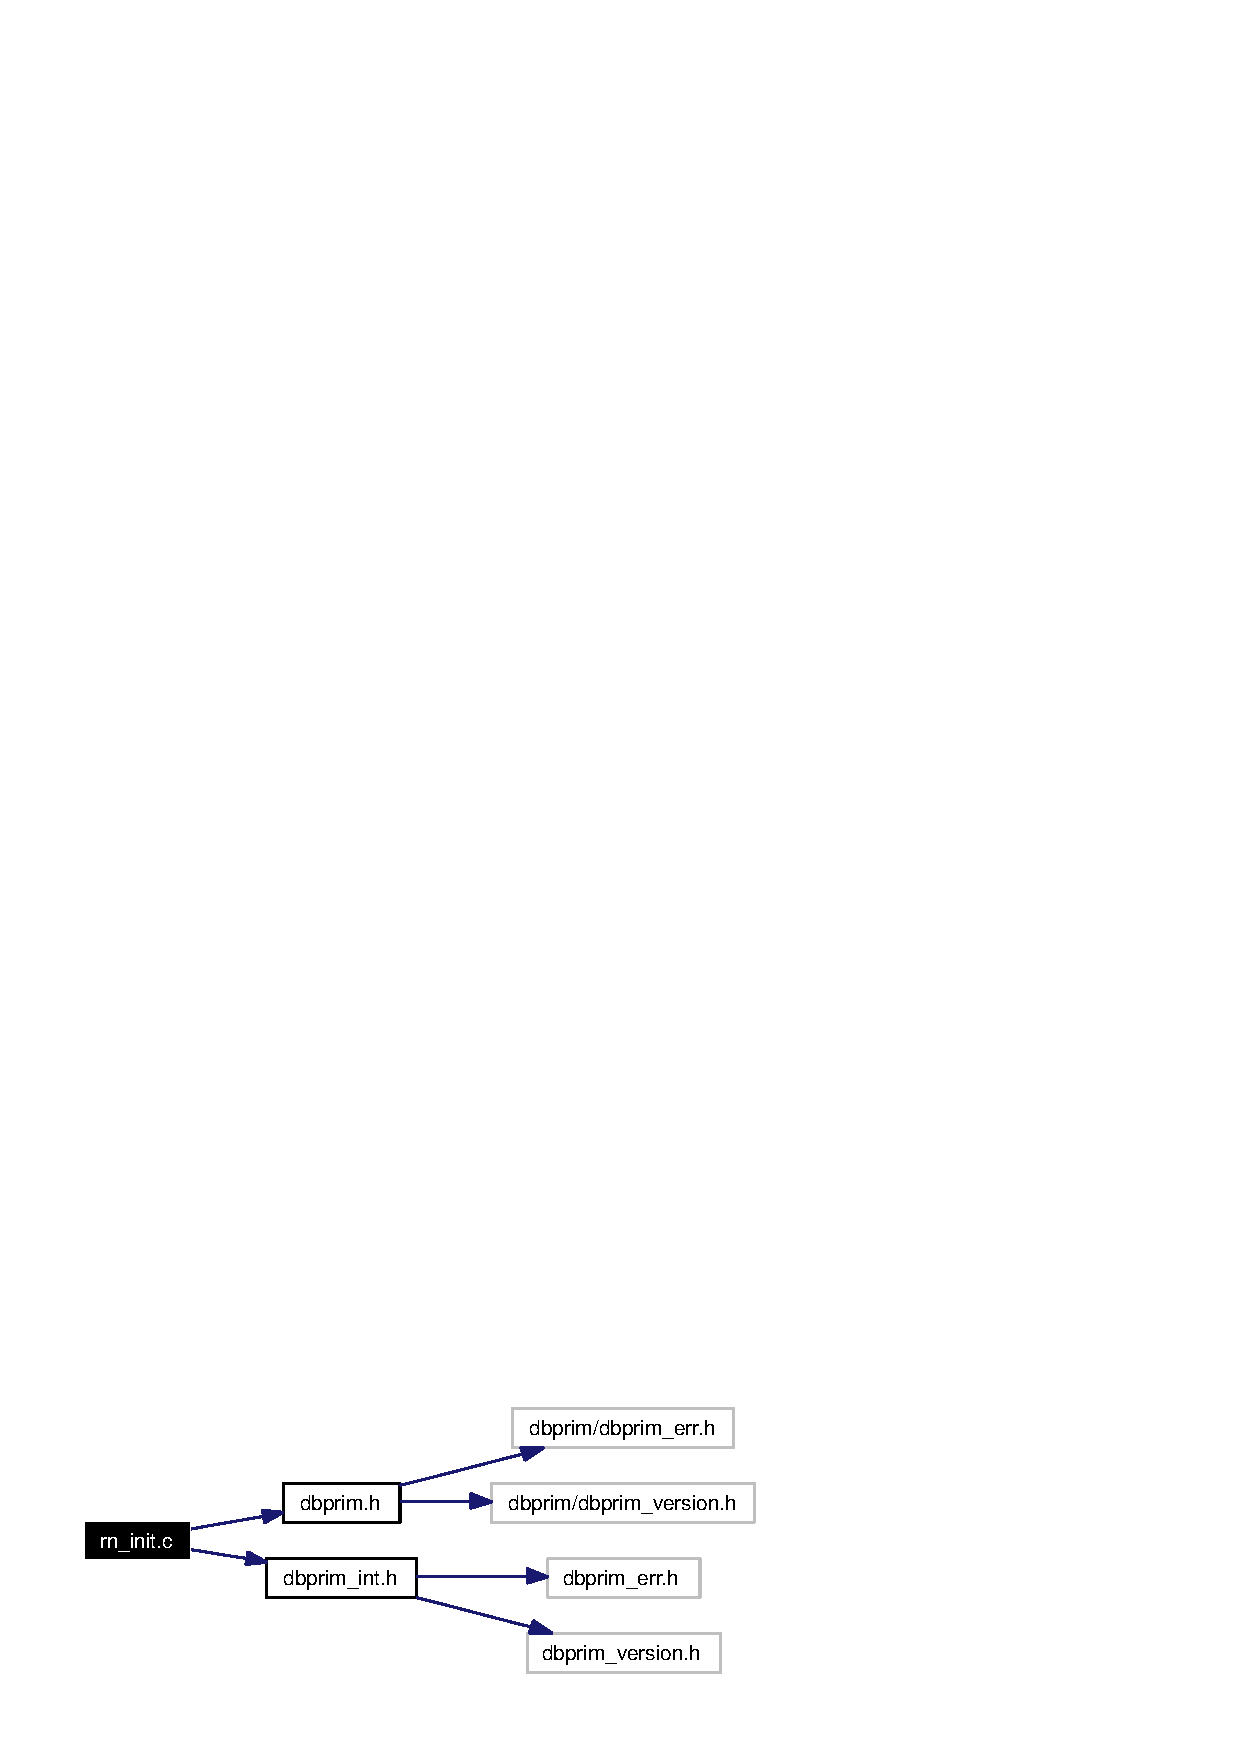
\includegraphics[width=183pt]{rn__init_8c__incl}
\end{center}
\end{figure}
\subsection*{Functions}
\begin{CompactItemize}
\item 
unsigned long \hyperlink{group__dbprim__rbtree_ga14}{rn\_\-init} (\hyperlink{struct__rb__node__s}{rb\_\-node\_\-t} $\ast$node, void $\ast$value)
\begin{CompactList}\small\item\em Dynamically initialize a red-black tree node. \item\end{CompactList}\end{CompactItemize}
